\documentclass{article}
\usepackage{cmap}
\usepackage[utf8]{inputenc}
\usepackage[english,ukrainian]{babel}
\usepackage{graphicx}
\usepackage{geometry}
\usepackage{listings}
\usepackage{float}
\usepackage{multicol}
\usepackage{amsmath}
\geometry{
	a4paper,
	left=20mm,
	right=20mm,
	top=15mm,
	bottom=15mm,
}
\lstset{
	language=c,
	tabsize=4,
	keepspaces,
	showstringspaces=false,
}
\graphicspath{ {./pictures} }
\setlength{\parindent}{4em}

\newcommand\subject{Основи електроніки}
\newcommand\lecturer{професор кафедри ПЗ \\ Фечан А.В.}
\newcommand\teacher{доцент кафедри ПЗ \\ Коцун В.І.}
\newcommand\mygroup{ПЗ-22}
\newcommand\lab{6}
\newcommand\theme{Дослідження мультивібратора}
\newcommand\purpose{Вивчити схему побудови симетричного мультивібратора
	(MB), дослідити його роботу в різних режимах}

\begin{document}
\begin{normalsize}
	\begin{titlepage}
		\thispagestyle{empty}
		\begin{center}
			\textbf{МІНІСТЕРСТВО ОСВІТИ І НАУКИ УКРАЇНИ\\
				НАЦІОНАЛЬНИЙ УНІВЕРСИТЕТ "ЛЬВІВСЬКА ПОЛІТЕХНІКА"}
		\end{center}
		\begin{flushright}
			\textbf{ІКНІ}\\
			Кафедра \textbf{ПЗ}
		\end{flushright}
		\vspace{200pt}
		\begin{center}
			\textbf{ЗВІТ}\\
			\vspace{10pt}
			до лабораторної роботи № \lab\\
			\textbf{на тему}: “\textit{\theme}”\\
			\textbf{з дисципліни}: “\subject”
		\end{center}
		\vspace{112pt}
		\begin{flushright}
			
			\textbf{Лектор}:\\
			\lecturer\\
			\vspace{28pt}
			\textbf{Виконав}:\\
			
			студент групи \mygroup\\
			Коваленко Д.М.\\
			\vspace{28pt}
			\textbf{Прийняв}:\\
			
			\teacher\\
			
			\vspace{28pt}
			«\rule{1cm}{0.15mm}» \rule{1.5cm}{0.15mm} 2023 р.\\
			$\sum$ = \rule{1cm}{0.15mm}……………\\
			
		\end{flushright}
		\vspace{\fill}
		\begin{center}
			\textbf{Львів — 2023}
		\end{center}
	\end{titlepage}
		
	\begin{description}
		\item[Тема.] \theme.
		\item[Мета.] \purpose.
	\end{description}

	\section*{Індивідуальне завдання}
	\begin{enumerate}
		\item Зберіть схему МВ в середовищі Multisim. Налаштуйте необхідні параметри моделювання і отримаєте осцилограми коливань МВ на базах і колекторах транзисторів. Визначте період коливань МВ і шпаруватість імпульсів
		\item Розрахуйте тривалості імпульсу Ті і паузи Тп по фор- мулів, наведеним вище, і порівняйте розрахункові результати з результатами, отриманими в п. 3.1.
		\item Дослідіть залежність періоду коливань МВ від номіналів конденсаторів C1 і C2. Для цього, змінюючи їх значення, визначте період коливань МВ, результати вимірювань зведіть в таблицю
		\item Аналогічно п.3, визначте залежність періоду коливань МВ від номіналів резисторів R1 і R2. Результати вимірювань зведіть в таблицю
		\item Поставте на стенді в схемі на (див. Рис. 8.2) конденсатори C1 і C2 різних номіналів. Визначте, як зміниться шпаруватість імпульсів. Результати зведіть в таблицю
		\item Дослідження роботи МВ в режимі синхронізації. У схемі, представленої на рис. 2, подайте на базу транзистора VT1 сигнал з генератора імпульсів (для версії Multisim 5.12 можна використовувати «Function generator»). Визначте, як змінюється частота коливань МВ зі зміною частоти імпульсів на виході синхронзвзуючого генератора. Результати вимірювань зведіть в таблицю
	\end{enumerate}

	\section*{Хід виконання}
	
	\begin{figure}[H]
		\centering
		\includegraphics[width=\textwidth]{1}
		\caption{Схема 1}
	\end{figure}

	\begin{figure}[H]
		\centering
		\includegraphics[width=\textwidth]{2}
		\caption{Осцилограма для схеми 1}
	\end{figure}

	\begin{multicols}{2}
		За даними осцилографа:
		\begin{gather}
			T_{\text{і}}=46.951\text{ мс}\nonumber\\
			T_{\text{п}}=46.970\text{ мс}\nonumber\\
			T=T_{\text{і}}+T_{\text{п}}=93.921\text{ мс}\nonumber
		\end{gather}
		
		\columnbreak
		
		За обрахунками:
		\begin{gather}
			T_{\text{і}}=46.41\text{ мс}\nonumber\\
			T_{\text{п}}=46.2\text{ мс}\nonumber\\
			T=T_{\text{і}}+T_{\text{п}}=92.61\text{ мс}\nonumber
		\end{gather}
	\end{multicols}

	\begin{table}[H]
		\centering
		\renewcommand*\arraystretch{1.3}
		\begin{tabular}{|p{0.12\linewidth}|p{0.08\linewidth}|p{0.08\linewidth}|p{0.08\linewidth}|p{0.08\linewidth}|p{0.08\linewidth}|}
			\hline
			$C$, $\mu F$&1&1.5&2&2.5&3\\
			\hline
			$T$, мс&42.8&64.0&85.6&106.4&127.25\\
			\hline
		\end{tabular}
		\caption{Таблиця залежності періоду коливань від ємностей $C_1$ та $C_2$}
	\end{table}
	
	\begin{table}[H]
		\centering
		\renewcommand*\arraystretch{1.3}
		\begin{tabular}{|p{0.12\linewidth}|p{0.08\linewidth}|p{0.08\linewidth}|p{0.08\linewidth}|p{0.08\linewidth}|p{0.08\linewidth}|}
			\hline
			$R$, $kOhm$&20&25&30&35&40\\
			\hline
			$T$, мс&62.88&78.4&93.2&109.0&125.0\\
			\hline
		\end{tabular}
		\caption{Таблиця залежності періоду коливань від величини $R_1$ та $R_2$}
	\end{table}
	
	\begin{table}[H]
		\centering
		\renewcommand*\arraystretch{1.3}
		\begin{tabular}{|p{0.12\linewidth}|p{0.08\linewidth}|p{0.08\linewidth}|p{0.08\linewidth}|p{0.08\linewidth}|p{0.08\linewidth}|}
			\hline
			$C_2$, $\mu F$&1&1.5&2&2.5&3\\
			\hline
			$T$, мс&68.5&78.4&89.8&100.0&110.6\\
			\hline
			$T_{\text{ні}}$, мс&21.0&31.4&42.8&53.0&64.0\\
			\hline
			$T_{\text{шп}}$&1.445&1.667&1.922&2.128&2.373\\
			\hline
		\end{tabular}
		\caption{Таблиця залежності шпаруватості імпульсів від ємності $C_2$}
	\end{table}
	
	\begin{figure}[H]
		\centering
		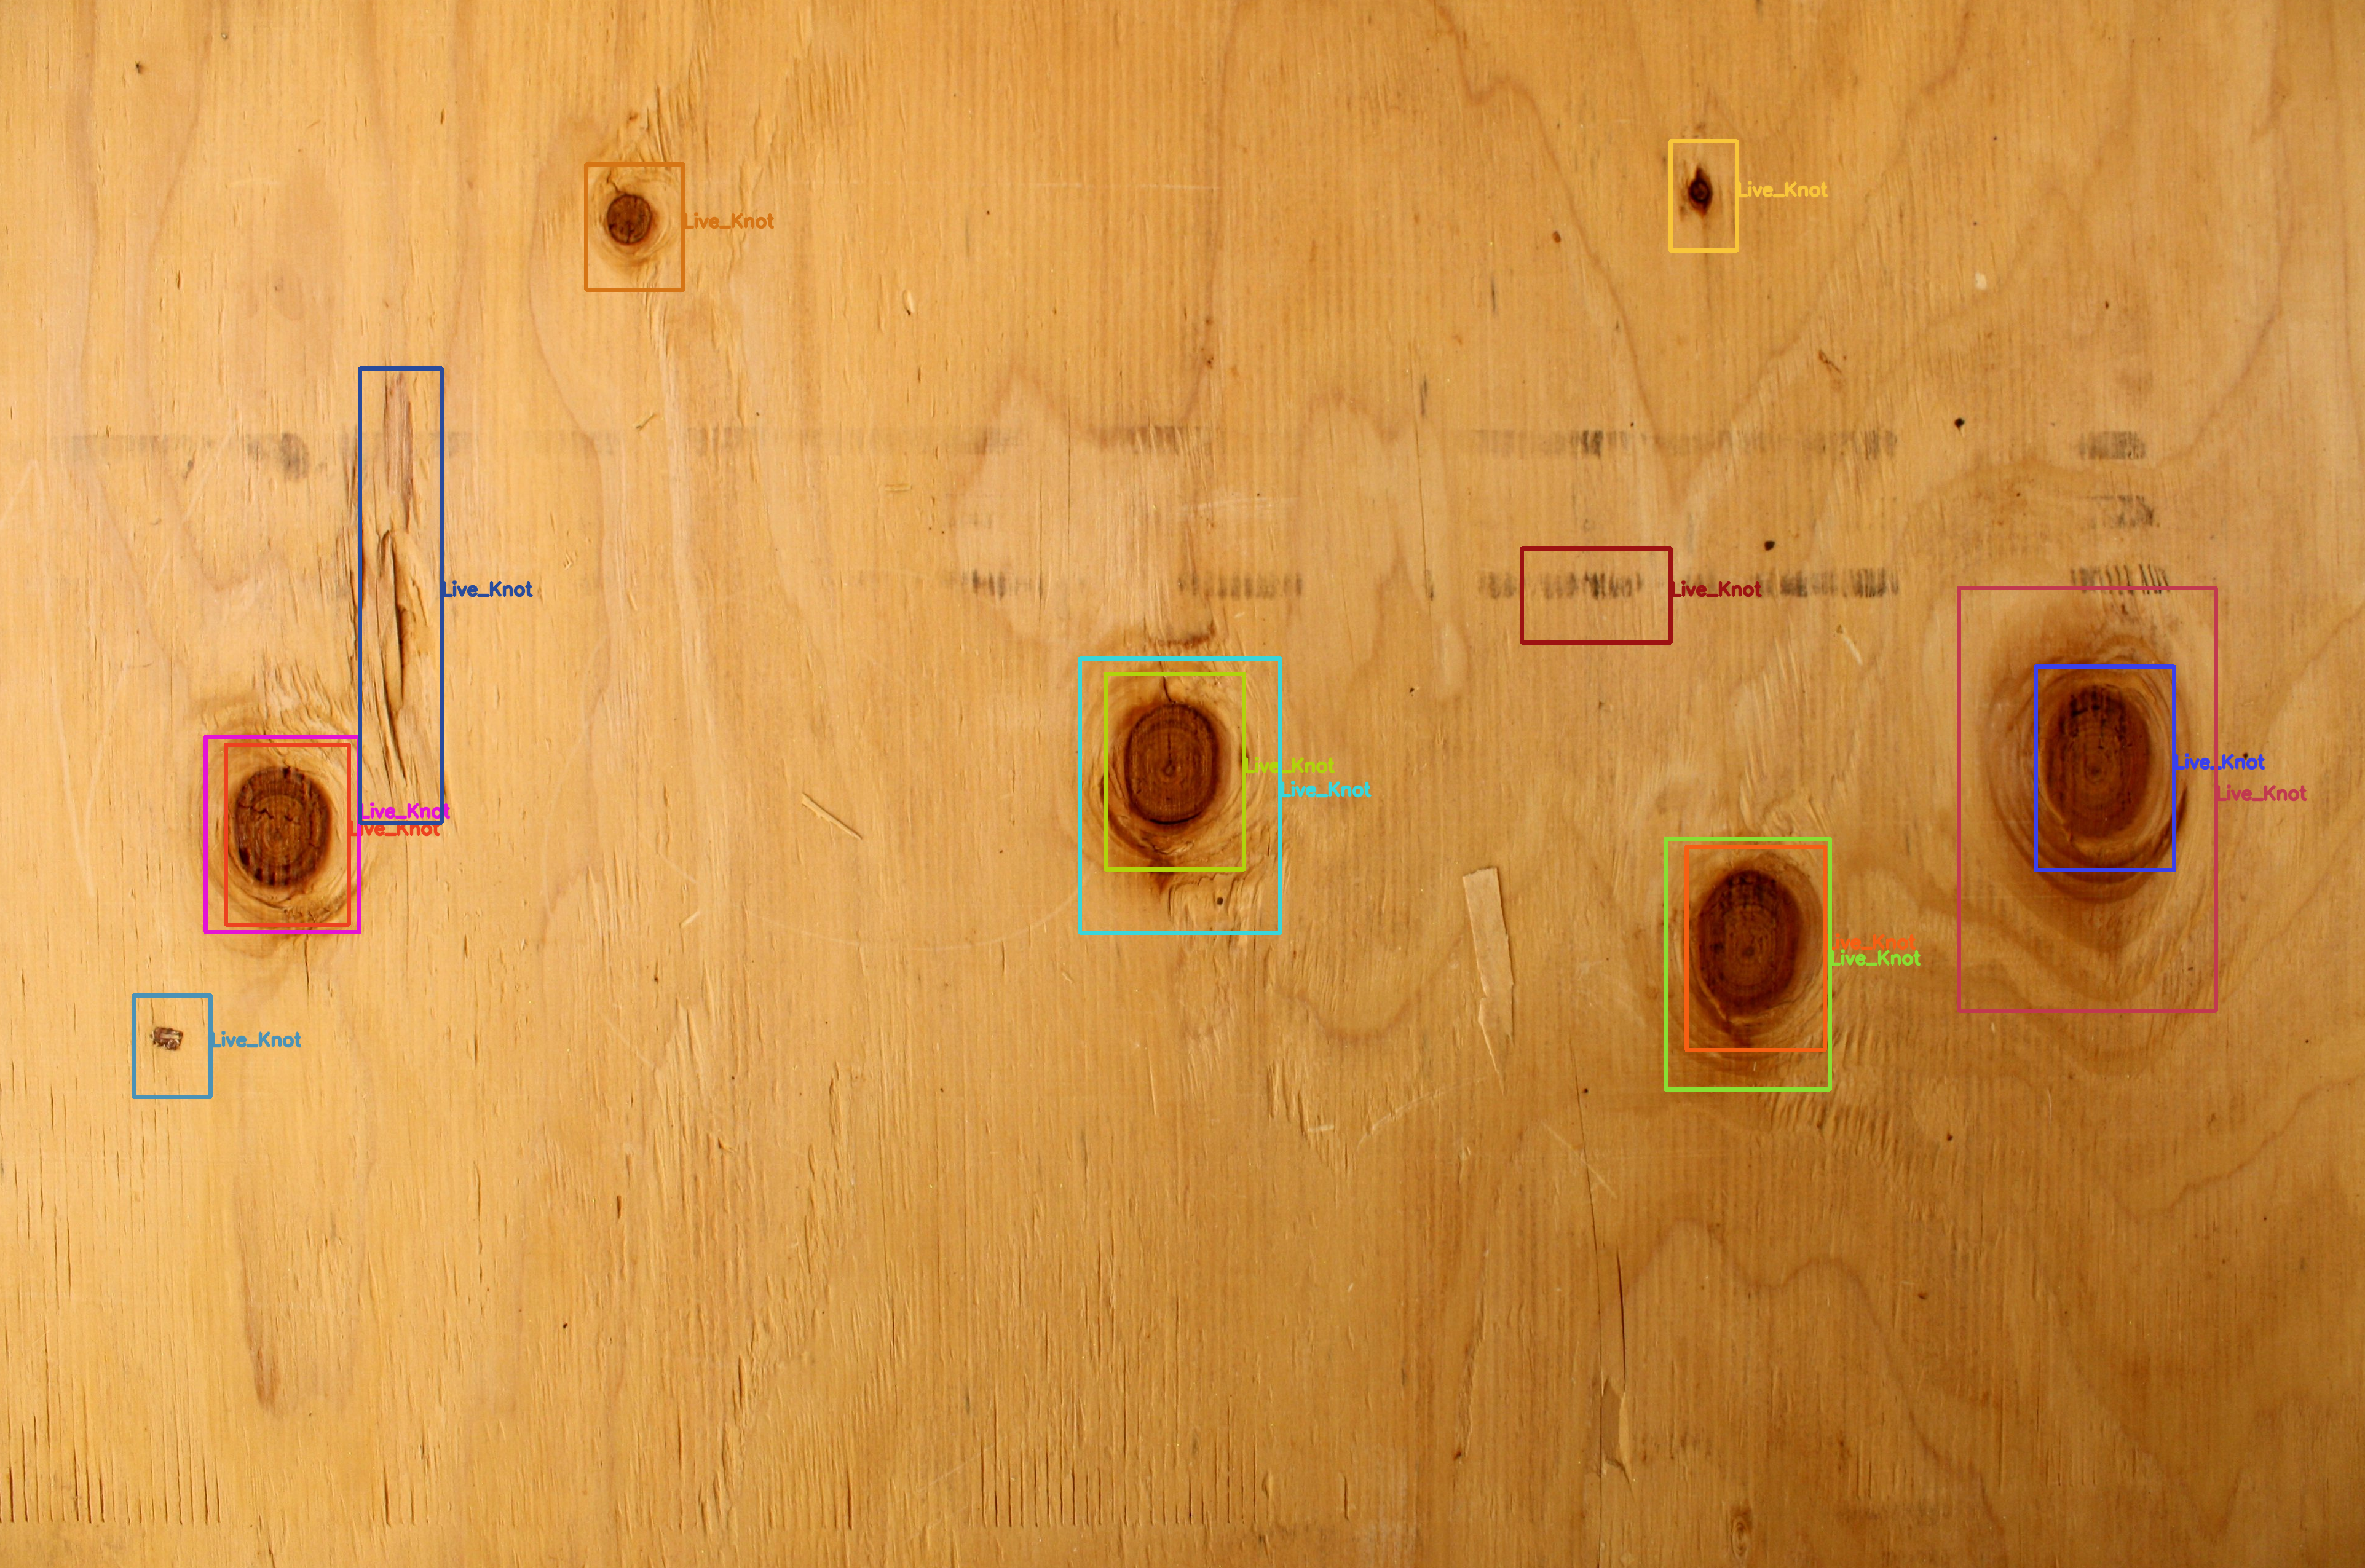
\includegraphics[width=\textwidth]{3}
		\caption{Схема 2}
	\end{figure}
	
	\begin{figure}[H]
		\centering
		\includegraphics[width=\textwidth]{4}
		\caption{Осцилограма для схеми 2}
	\end{figure}
	
	\begin{table}[H]
		\centering
		\renewcommand*\arraystretch{1.3}
		\begin{tabular}{|p{0.12\linewidth}|p{0.08\linewidth}|p{0.08\linewidth}|p{0.08\linewidth}|p{0.08\linewidth}|p{0.08\linewidth}|}
			\hline
			$F_{r_{\text{г}}}$, $Hz$&1&5&10&20&30\\
			\hline
			$F_{r_{\text{МВ}}}$, $Hz$&1&5&10&20&30\\
			\hline
		\end{tabular}
		\caption{Таблиця залежності періоду коливань від величини $R_1$ та $R_2$}
	\end{table}
	
	\section*{Висновки}
	Під час виконання лабораторної роботи я вивчив схему побудови симетричного мультивібратора
	(MB), дослідив його роботу в різних режимах.
	    
\end{normalsize}
\end{document}
